\section{Static Force/Torque Relationships}

\begin{frame}[standout, plain, noframenumbering]
    Static Force/Torque Relationships

    % \medskip

    % \footnotesize
    % Sam Greydanus \quad Misko Dzamba \quad Jason Yosinski
\end{frame}

\begingroup
\small


\begin{frame}
    \frametitle{Static Force/Torque Relationships}

    \begin{itemize}
        \item Interaction of the manipulator with the environment produces
        forces and moments at the end effector or tool.
        \item These produce torques at the joints of the robot.\footnotemark
        \item We discuss the role of the manipulator Jacobian in the
        quantitative relationship between the end effector forces and joint
        torques.
        \item Let $F = (F_x, F_y, F_z, n_x, n_y, n_z)$ represent the vector of 
        forces and moments at the end effector.
        \item Let $\tau$ denote the corresponding vector of joint torques. Then 
        \begin{equation}
            \boxed{\tau = J^\top(q) F.}
            \label{eq:static_force_torque}
        \end{equation} 
    \end{itemize}

    \footnotetext{We consider only revolute joints. If the joints are prismatic, 
    forces and moments at the end effector produce forces at the joints.}
\end{frame}


\begin{frame}
    \frametitle{Static Force/Torque Relationships}

    \begin{itemize}
        \item We derive the relationship~\eqref{eq:static_force_torque} through 
        the so-called \textbf{principle of virtual work}.
        \item Its detailed discussion is deferred. Instead an informal
        justification follows.
        \item Let $\delta X$ and $\delta q$ represent infinitesimal
        displacements in the task space and joint space, respectively.
        \item These displacements are called \textbf{virtual displacements} if 
        they are consistent with any constraints imposed on the system.
        \item For example, if the end effector is in contact with a rigid wall, 
        then the virtual displacements in position are tangent to the wall.
        \item These virtual displacements are related through the manipulator 
        Jacobian $J(q)$ according to 
        \begin{equation}
            \delta X = J(q) \delta q.
            \label{eq:virtual_displacement}
        \end{equation}
    \end{itemize}
\end{frame}


\begin{frame}
    \frametitle{Static Force/Torque Relationships}

    \begin{itemize}
        \item The virtual work $\delta w$ of the system is 
        \[ \delta w = F^\top \delta X - \tau^\top \delta q. \]
        \item Substituting equation~\eqref{eq:virtual_displacement} into the
        equation above yields
        \begin{equation}
            \delta w = \left( F^\top J - \tau^\top \right) \delta q.
            \label{eq:force_torque}
        \end{equation} 
        \item The principle of virtual work says that the quantity given by
        equation~\eqref{eq:force_torque} is equal to zero if the manipulator is
        in equilibrium. This gives rise to the
        equation~\eqref{eq:static_force_torque}.
    \end{itemize}
\end{frame}



\begin{frame}
    \frametitle{Example: Two-Link Planar Manipulator}

    \begin{columns}
        \begin{column}{0.6\textwidth}
            \begin{itemize}
                \item A force $F$ is applied at the end of link $2$ as shown.
                \item The Jacobian of this manipulator was formulated earlier.
                \item The resulting joint torques $\tau = (\tau_1, \tau_2)$ are 
                then given by 
            \end{itemize}
        \end{column}
        \begin{column}{0.4\textwidth}
            \begin{figure}[bth]
                \centering
                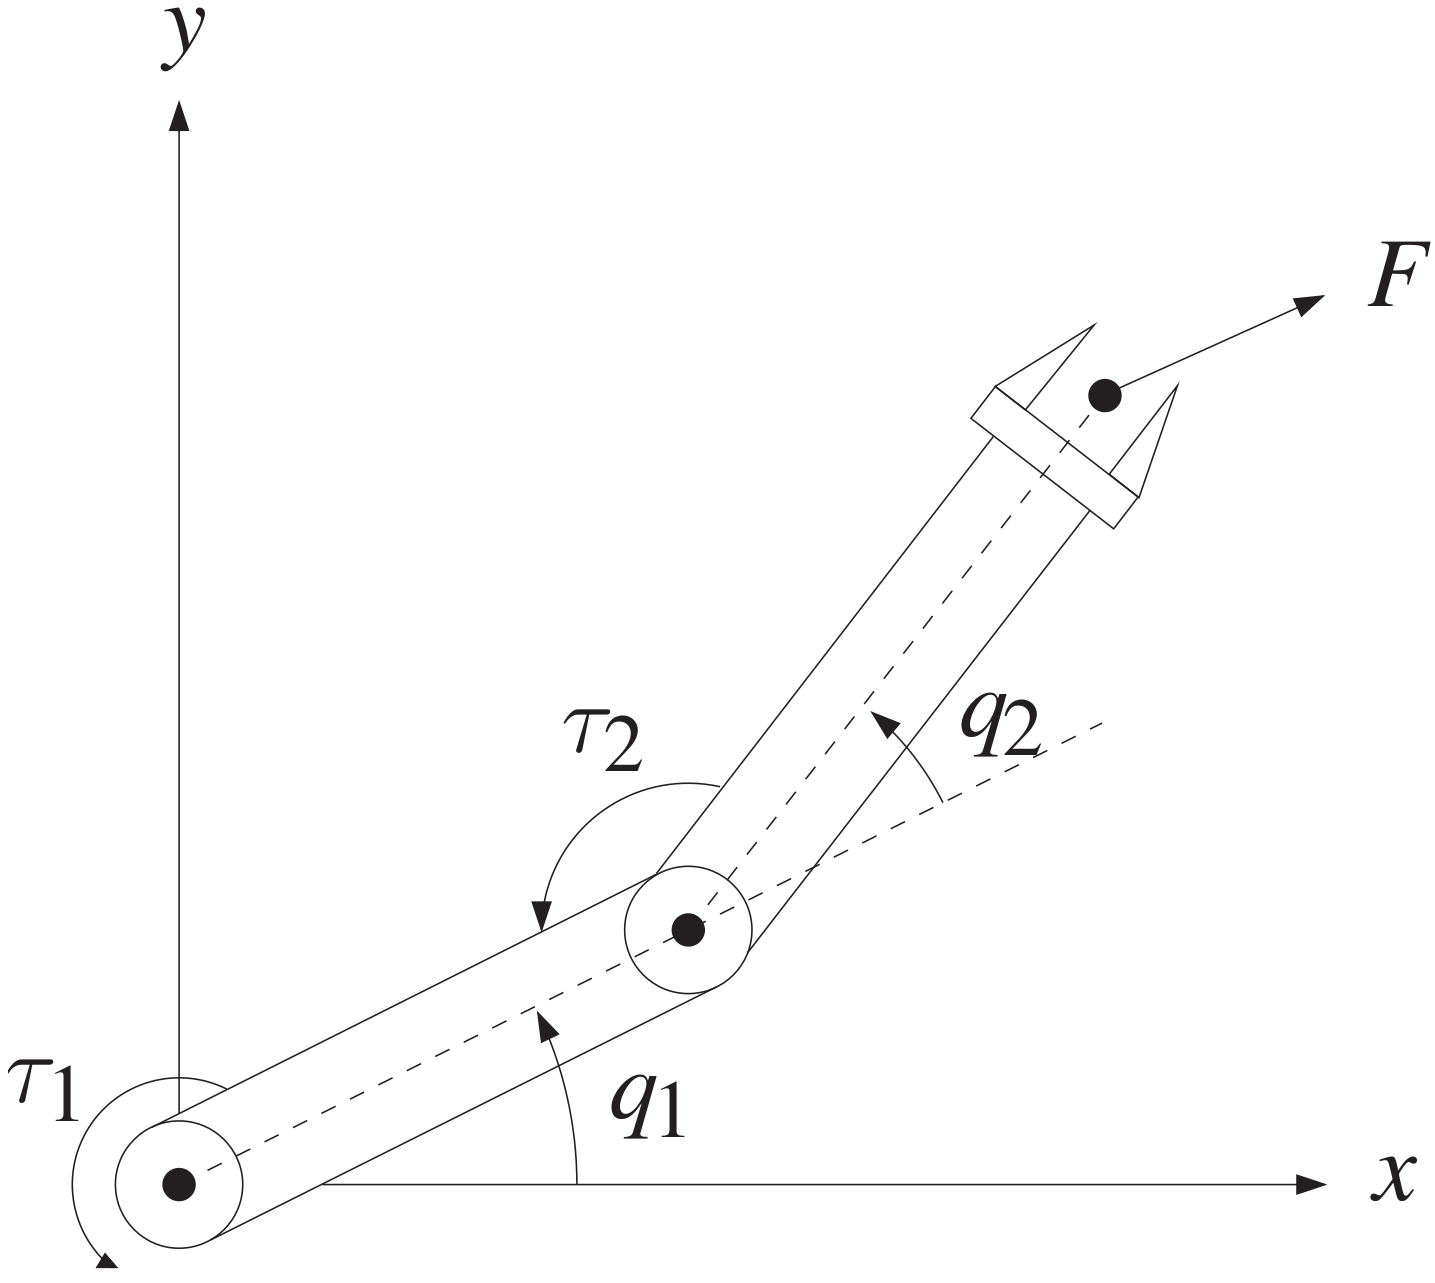
\includegraphics[width=0.85\textwidth]{figures/two_link_robot.png} 
                % \caption{\footnotesize }
            \end{figure}
            \vspace{-2mm}
            \centering
            \footnotesize{Two-link planar robot.}
        \end{column}
    \end{columns}
    \[
    \bmat{\tau_1 \\ \tau_2} = \bmat{
        -a_1s_1 - a_2s_{12} & a_1c_1 + a_2c_{12} & 0 & 0 & 0 & 1 \\ 
        -a_2s_{12} & a_2c_{12} & 0 & 0 & 0 & 1
    }\bmat{F_x \\ F_y \\ F_z \\ n_x \\ n_y \\ n_z}.
    \]
\end{frame}


\endgroup